%=================================================================
% CSE 4345 — Big Data Analytics
% Week 9, Part 2: Seminal Research & Case Study
% Department of CSE, Premier University
%
% SEMINAL WORKS:
%   Tufte, E. R. (1983) — The Visual Display of Quantitative
%   Information. Graphics Press. (cited >20,000 times)
%
%   Shneiderman, B. (1996) — The Eyes Have It: A Task by Data
%   Type Taxonomy for Information Visualizations.
%   IEEE VL 1996. (cited >5,000 times)
%
% CASE STUDY:
%   New York Times Graphics Desk (2010–2022): D3.js, award-winning
%   interactive journalism, COVID-19 visualisations
%=================================================================

\documentclass[aspectratio=169,10pt]{beamer}

%---------- Packages ----------
\usepackage[utf8]{inputenc}
\usepackage[T1]{fontenc}
\usepackage{booktabs}
\usepackage{xcolor}
\usepackage{tikz}
\usetikzlibrary{shapes.geometric, positioning, arrows.meta,
                decorations.pathreplacing}
\usepackage{amsmath}
\usepackage{graphicx}
\usepackage{multicol}
\usepackage{enumerate}
\usepackage{array}

%---------- Theme ----------
\usetheme{Madrid}

%---------- Premier University Color Identity ----------
\definecolor{PUNavy}{RGB}{10,36,99}
\definecolor{PUGold}{RGB}{197,151,37}
\definecolor{PULightBlue}{RGB}{210,228,255}
\definecolor{PUTeal}{RGB}{0,100,100}
\definecolor{PUGray}{RGB}{90,90,90}
\definecolor{PURed}{RGB}{160,30,30}
\definecolor{PUGreen}{RGB}{30,120,60}
\definecolor{PUPurple}{RGB}{90,30,120}
\definecolor{PUOrange}{RGB}{190,90,20}

\setbeamercolor{palette primary}{bg=PUNavy, fg=white}
\setbeamercolor{palette secondary}{bg=PUNavy!85, fg=white}
\setbeamercolor{palette tertiary}{bg=PUNavy!70, fg=white}
\setbeamercolor{palette quaternary}{bg=PUNavy, fg=white}
\setbeamercolor{structure}{fg=PUNavy}
\setbeamercolor{title}{bg=PUNavy, fg=PUGold}
\setbeamercolor{subtitle}{fg=white}
\setbeamercolor{frametitle}{bg=PUNavy, fg=PUGold}
\setbeamercolor{alerted text}{fg=PUGold!85!black}
\setbeamercolor{block title}{bg=PUNavy, fg=white}
\setbeamercolor{block body}{bg=PULightBlue!45}
\setbeamercolor{block title alerted}{bg=PUGold!80!black, fg=white}
\setbeamercolor{block body alerted}{bg=PUGold!12}
\setbeamercolor{block title example}{bg=PUTeal, fg=white}
\setbeamercolor{block body example}{bg=PUTeal!10}
\setbeamercolor{section in toc}{fg=PUNavy}
\setbeamercolor{itemize item}{fg=PUGold!80!black}
\setbeamercolor{itemize subitem}{fg=PUNavy!70}

\setbeamertemplate{navigation symbols}{}
\setbeamertemplate{itemize item}{\scriptsize\raise1.5pt\hbox{\textbullet}}
\setbeamertemplate{itemize subitem}{\scriptsize\raise1pt\hbox{--}}

%---------- Section separator ----------
\AtBeginSection[]{
  \begin{frame}[plain]
    \vfill
    \centering
    \begin{beamercolorbox}[sep=12pt,center,shadow=true,rounded=true]{block title}
      \usebeamerfont{title}\insertsectionhead\par
    \end{beamercolorbox}
    \vfill
  \end{frame}
}

%---------- Helper: citation box ----------
\newenvironment{paperbox}[1]{%
  \setbeamercolor{block title}{bg=PUNavy!90,fg=PUGold}
  \setbeamercolor{block body}{bg=PUNavy!6}
  \begin{block}{#1}}{%
  \end{block}}

%---------- Custom footline ----------
\setbeamertemplate{footline}{
  \leavevmode\hbox{%
    \begin{beamercolorbox}[wd=.333\paperwidth,ht=2.25ex,dp=1ex,center]{palette primary}
      \usebeamerfont{author in head/foot}\insertshortauthor
    \end{beamercolorbox}%
    \begin{beamercolorbox}[wd=.334\paperwidth,ht=2.25ex,dp=1ex,center]{palette secondary}
      \usebeamerfont{title in head/foot}\insertshorttitle
    \end{beamercolorbox}%
    \begin{beamercolorbox}[wd=.333\paperwidth,ht=2.25ex,dp=1ex,right]{palette primary}
      \usebeamerfont{date in head/foot}
      \insertframenumber{} / \inserttotalframenumber\hspace*{2ex}
    \end{beamercolorbox}}%
  \vskip0pt%
}

%---------- Title metadata ----------
\title[CSE 4345 \textbar{} Week 9, Part 2]{CSE 4345: Big Data Analytics}
\subtitle{Week 9, Part 2 \textemdash\ Seminal Research \& Case Study}
\author[Dept.\ of CSE]{Department of Computer Science \& Engineering\\[4pt]
       \small Premier University, Chittagong}
\institute{}
\date{Semester 2026}

%=================================================================
\begin{document}
%=================================================================

%----------------------------------------------------------------
\begin{frame}
  \titlepage
\end{frame}

%----------------------------------------------------------------
\begin{frame}{Part 2 Overview — Week 9}
  \begin{columns}[T]
    \column{0.47\textwidth}
      \begin{block}{Today's Agenda}
        \tableofcontents
      \end{block}
    \column{0.50\textwidth}
      \begin{exampleblock}{Seminal Works Covered}
        \begin{enumerate}
          \item Tufte, E.~R. (1983).
                \textit{The Visual Display of Quantitative
                Information.} Graphics Press.
          \item Shneiderman, B. (1996).
                \textit{The Eyes Have It: A Task by Data Type
                Taxonomy for Information Visualizations.}
                IEEE Visual Languages.
        \end{enumerate}
      \end{exampleblock}
      \vspace{6pt}
      \begin{alertblock}{Case Study}
        New York Times Graphics Desk (2010--2022):
        interactive data journalism using D3.js, reaching
        \textbf{6 million readers per day}; COVID-19
        visualisations cited in policy briefs worldwide.
      \end{alertblock}
      \vspace{4pt}
      \begin{block}{CLO Addressed}
        \textbf{CLO3} — Explain data visualisation principles\\
        \textbf{PLO(b)}
      \end{block}
  \end{columns}
\end{frame}

%================================================================
\section{Work 1 — Tufte (1983): The Visual Display of Quantitative Information}
%================================================================

%----------------------------------------------------------------
\begin{frame}{Research Landscape: History of Data Visualisation}
  \begin{center}
  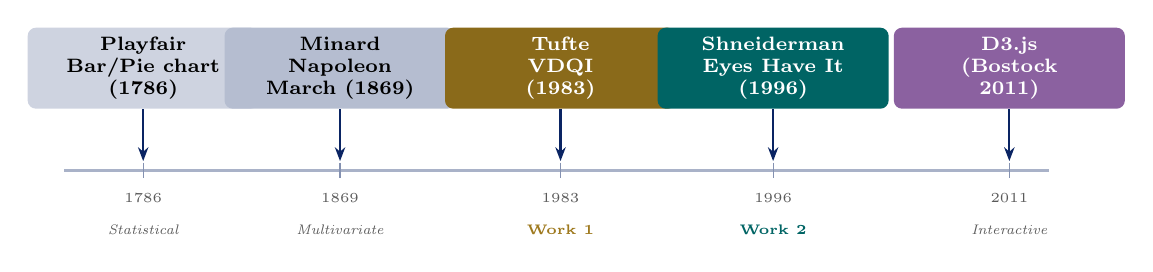
\begin{tikzpicture}[
      nbox/.style={rectangle, rounded corners=3pt, minimum width=2.9cm,
                   minimum height=0.9cm, text width=2.7cm, align=center,
                   font=\scriptsize\bfseries},
      arr/.style={-{Stealth[length=5pt]}, draw=PUNavy, thick}
    ]
    \draw[PUNavy!35, very thick] (0,0) -- (12.5,0);

    \node[nbox, fill=PUNavy!20]              (play) at (1.0, 1.3)
          {Playfair\\Bar/Pie chart\\(1786)};
    \node[nbox, fill=PUNavy!30]              (min)  at (3.5, 1.3)
          {Minard\\Napoleon\\March (1869)};
    \node[nbox, fill=PUGold!70!black, text=white] (tuf) at (6.3, 1.3)
          {Tufte\\VDQI\\(1983)};
    \node[nbox, fill=PUTeal, text=white]     (shn)  at (9.0, 1.3)
          {Shneiderman\\Eyes Have It\\(1996)};
    \node[nbox, fill=PUPurple!70, text=white](d3)   at (12.0,1.3)
          {D3.js\\(Bostock\\2011)};

    \foreach \x/\y in {1.0/1786, 3.5/1869, 6.3/1983, 9.0/1996, 12.0/2011}{
      \draw[PUNavy!50] (\x,0.1) -- (\x,-0.1);
      \node[font=\tiny, text=PUGray] at (\x,-0.35) {\y};
    }

    \draw[arr] (play) -- (1.0,  0.12);
    \draw[arr] (min)  -- (3.5,  0.12);
    \draw[arr] (tuf)  -- (6.3,  0.12);
    \draw[arr] (shn)  -- (9.0,  0.12);
    \draw[arr] (d3)   -- (12.0, 0.12);

    \node[font=\tiny\itshape, text=PUGray]           at (1.0,  -0.75) {Statistical};
    \node[font=\tiny\itshape, text=PUGray]           at (3.5,  -0.75) {Multivariate};
    \node[font=\tiny\bfseries, text=PUGold!80!black] at (6.3,  -0.75) {Work 1};
    \node[font=\tiny\bfseries, text=PUTeal]          at (9.0,  -0.75) {Work 2};
    \node[font=\tiny\itshape, text=PUGray]           at (12.0, -0.75) {Interactive};
  \end{tikzpicture}
  \end{center}
  \vspace{4pt}
  \begin{alertblock}{Why Tufte Matters for Big Data Visualisation}
    Big Data pipelines produce outputs humans must interpret.
    A chart with \textbf{chartjunk} on a 4K dashboard misleads
    as badly as a bad statistical test.
    Tufte's principles are the analytical foundation for every
    modern dashboard framework (Tableau, Grafana, D3).
    The week's D3 practicals are applications of Tufte's rules.
  \end{alertblock}
\end{frame}

%----------------------------------------------------------------
\begin{frame}{Tufte (1983): Publication Context}
  \begin{columns}[T]
    \column{0.53\textwidth}
      \begin{paperbox}{Full Citation}
        Tufte, E.~R. (1983).
        \textbf{The Visual Display of Quantitative Information.}
        Graphics Press, Cheshire, CT.
        (2nd ed., 2001; 197 pp.)\\[5pt]
        \textbf{Format:} Book (self-published by Tufte;
        designed and typeset by Tufte himself)\\
        \textbf{Cited by:} $>$20{,}000 (Google Scholar, 2024)\\
        \textbf{Author:} Edward R.\ Tufte, Professor of Statistics,
        Graphic Design, and Political Economy (Yale University)\\[4pt]
        \textbf{Note}: the book was \emph{rejected by every publisher}
        Tufte approached; he mortgaged his house to self-publish.
        It sold 40{,}000 copies in its first year.
      \end{paperbox}
      \vspace{5pt}
      \begin{exampleblock}{Tufte's Central Claim}
        \begin{center}
        \large\color{PUNavy}
        \textit{``Graphical excellence is that which
        gives to the viewer the greatest number of ideas
        in the shortest time with the least ink
        in the smallest space.''}
        \end{center}
      \end{exampleblock}

    \column{0.44\textwidth}
      \begin{block}{The Context: Why 1983?}
        \begin{itemize}
          \item By 1983, computer-generated charts were proliferating
                in corporate reports and newspapers
          \item Most were produced by software that defaulted to
                heavy gridlines, 3-D effects, unnecessary colour,
                and excessive labelling
          \item Tufte analysed \textbf{4{,}000 charts} from science,
                business, and journalism publications to identify
                patterns of effective and deceptive design
          \item His contemporaries focused on \emph{how to draw}
                charts; Tufte focused on \emph{what to show}
                and \emph{what to remove}
        \end{itemize}
      \end{block}
  \end{columns}
\end{frame}

%----------------------------------------------------------------
\begin{frame}{Technical Contribution 1 — Data-Ink Ratio \& Chartjunk}
  \begin{columns}[T]
    \column{0.50\textwidth}
      \begin{block}{The Data-Ink Ratio}
        \[
          \text{Data-Ink Ratio} =
          \frac{\text{ink used to display data}}
               {\text{total ink used in the graphic}}
        \]
        \textbf{Goal}: maximise data-ink ratio.
        Every non-data mark must justify its existence.\\[5pt]
        \textbf{Chartjunk} — Tufte's term for ink that does not
        convey data:
        \begin{itemize}
          \item \textbf{Vibrations}: optical illusions from
                cross-hatching and dense patterns
          \item \textbf{Grids}: heavy gridlines compete with data;
                use light or no gridlines
          \item \textbf{Ducks}: graphic elements that represent
                themselves rather than data
                (e.g., a chart drawn as a 3-D bar on a fake desktop)
          \item \textbf{3-D effects}: depth, shadows, and perspective
                distort quantitative comparisons — never use 3-D
                for 2-D data
        \end{itemize}
      \end{block}

    \column{0.47\textwidth}
      \begin{center}
      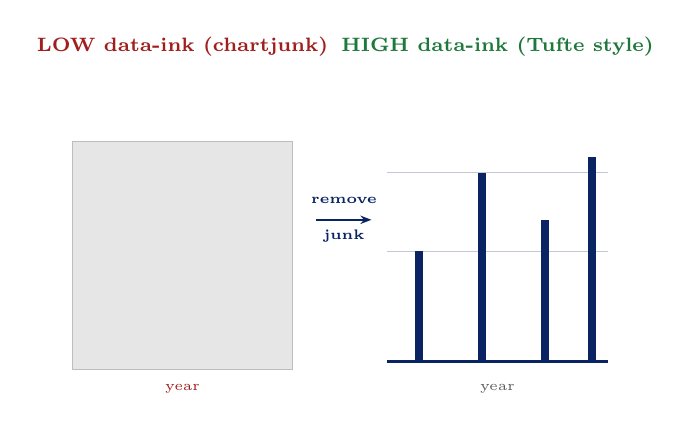
\begin{tikzpicture}[
          arr/.style={-{Stealth[length=4pt]}, draw=PUNavy, thick}
        ]
        %--- Before: low data-ink (chartjunk) ---
        \node[font=\scriptsize\bfseries, text=PURed] at (-1.8, 4.4)
              {LOW data-ink (chartjunk)};

        % Heavy grid
        \foreach \y in {0.6, 1.2, 1.8, 2.4, 3.0} {
          \draw[PUGray!60, line width=1.0pt] (-3.2,\y) -- (-0.4,\y);
        }
        % 3-D bars (faked with thick rules)
        \draw[PUNavy!60, line width=8pt]  (-2.8, 0.4) -- (-2.8, 1.8);
        \draw[PUNavy!40, line width=8pt]  (-2.0, 0.4) -- (-2.0, 2.8);
        \draw[PUNavy!60, line width=8pt]  (-1.2, 0.4) -- (-1.2, 2.2);
        \draw[PUNavy!40, line width=8pt]  (-0.6, 0.4) -- (-0.6, 3.0);
        % Baseline
        \draw[PUNavy, thick] (-3.2, 0.4) -- (-0.4, 0.4);
        % Shadow box (chartjunk)
        \draw[PUGray!40, fill=PUGray!15]
              (-3.2, 0.3) rectangle (-0.4, 3.2);
        \node[font=\tiny, text=PURed] at (-1.8, 0.05) {year};

        %--- After: high data-ink ---
        \node[font=\scriptsize\bfseries, text=PUGreen] at (2.2, 4.4)
              {HIGH data-ink (Tufte style)};

        \draw[PUNavy!25, line width=0.4pt] (0.8, 1.8) -- (3.6, 1.8);
        \draw[PUNavy!25, line width=0.4pt] (0.8, 2.8) -- (3.6, 2.8);

        \draw[PUNavy, line width=3pt]  (1.2, 0.4) -- (1.2, 1.8);
        \draw[PUNavy, line width=3pt]  (2.0, 0.4) -- (2.0, 2.8);
        \draw[PUNavy, line width=3pt]  (2.8, 0.4) -- (2.8, 2.2);
        \draw[PUNavy, line width=3pt]  (3.4, 0.4) -- (3.4, 3.0);
        \draw[PUNavy, thick] (0.8, 0.4) -- (3.6, 0.4);
        \node[font=\tiny, text=PUGray] at (2.2, 0.05) {year};

        % Arrow between
        \draw[arr] (-0.1, 2.2) -- (0.6, 2.2);
        \node[font=\tiny\bfseries, text=PUNavy] at (0.25, 2.45)
              {remove};
        \node[font=\tiny\bfseries, text=PUNavy] at (0.25, 2.0)
              {junk};
      \end{tikzpicture}
      \end{center}
  \end{columns}
\end{frame}

%----------------------------------------------------------------
\begin{frame}{Technical Contribution 2 — Lie Factor, Small Multiples \& Sparklines}
  \begin{columns}[T]
    \column{0.50\textwidth}
      \begin{block}{The Lie Factor}
        \[
          \text{Lie Factor} =
          \frac{\text{size of effect shown in graphic}}
               {\text{size of effect in data}}
        \]
        A lie factor of 1 is truthful.
        $>$1: graphic \emph{overstates} the effect.
        $<$1: graphic \emph{understates} it.\\[4pt]
        \textbf{Classic example}: a bar chart where the $y$-axis
        starts at 50 instead of 0.
        If the data effect is $+10\%$ but the bar appears to double
        in height, the lie factor is $\approx 10$.
      \end{block}
      \vspace{5pt}
      \begin{block}{Small Multiples}
        The same chart structure repeated across many subsets of data.
        \begin{itemize}
          \item Enables \textbf{immediate visual comparison}
                across conditions, time, or geography
          \item Eliminates animation (which forces the viewer to remember
                the previous frame)
          \item Example: 12 monthly temperature line charts
                arranged in a $3 \times 4$ grid
        \end{itemize}
      \end{block}

    \column{0.47\textwidth}
      \begin{center}
      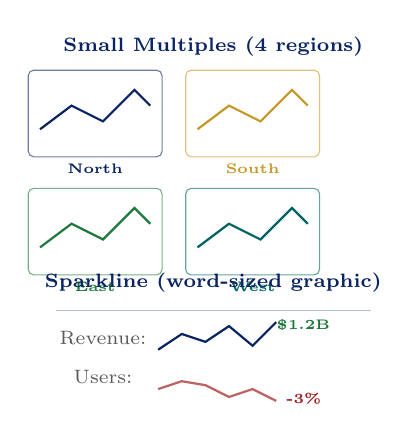
\begin{tikzpicture}[
          arr/.style={-{Stealth[length=3pt]}, draw=PUNavy, thick}
        ]
        %--- Small multiples illustration ---
        \node[font=\scriptsize\bfseries, text=PUNavy] at (0, 4.55)
              {Small Multiples (4 regions)};

        \foreach \cx/\cy/\col/\lbl in {
            -1.5/3.7/PUNavy/North,
             0.5/3.7/PUGold/South,
            -1.5/2.2/PUGreen/East,
             0.5/2.2/PUTeal/West}{
          \draw[\col!60, rounded corners=2pt]
                (\cx-0.85,\cy-0.55) rectangle (\cx+0.85,\cy+0.55);
          \draw[\col, thick]
                (\cx-0.7,\cy-0.2) -- (\cx-0.3,\cy+0.1)
                -- (\cx+0.1,\cy-0.1) -- (\cx+0.5,\cy+0.3)
                -- (\cx+0.7,\cy+0.1);
          \node[font=\tiny\bfseries, text=\col] at (\cx, \cy-0.7) {\lbl};
        }

        %--- Sparkline illustration ---
        \draw[PUNavy!30] (-2.0, 1.2) -- (2.0, 1.2);
        \node[font=\scriptsize\bfseries, text=PUNavy] at (0, 1.55)
              {Sparkline (word-sized graphic)};

        \node[font=\scriptsize, text=PUGray] at (-1.4, 0.85)
              {Revenue:};
        \draw[PUNavy, thick]
              (-0.7,0.7) -- (-0.4,0.9) -- (-0.1,0.8)
              -- (0.2,1.0) -- (0.5,0.75) -- (0.8,1.05);
        \node[font=\tiny\bfseries, text=PUGreen] at (1.15, 1.02)
              {\$1.2B};

        \node[font=\scriptsize, text=PUGray] at (-1.4, 0.35)
              {Users:};
        \draw[PURed!70, thick]
              (-0.7,0.2) -- (-0.4,0.3) -- (-0.1,0.25)
              -- (0.2,0.1) -- (0.5,0.2) -- (0.8,0.05);
        \node[font=\tiny\bfseries, text=PURed] at (1.15, 0.08)
              {-3\%};
      \end{tikzpicture}
      \end{center}
      \vspace{4pt}
      \begin{exampleblock}{Sparklines (Tufte 2006)}
        \textbf{Sparklines} are intense, simple, word-sized graphics
        embedded in text.  Grafana and Bloomberg terminals both
        implement sparklines — a direct application of Tufte's concept.
      \end{exampleblock}
  \end{columns}
\end{frame}

%================================================================
\section{Work 2 — Shneiderman (1996): The Eyes Have It}
%================================================================

%----------------------------------------------------------------
\begin{frame}{Shneiderman (1996): Publication Context \& the Mantra}
  \begin{columns}[T]
    \column{0.53\textwidth}
      \begin{paperbox}{Full Citation}
        Shneiderman, B. (1996).
        \textbf{The Eyes Have It: A Task by Data Type Taxonomy
        for Information Visualizations.}
        In \textit{Proceedings of the IEEE Symposium on Visual
        Languages}, pp.~336--343.
        Boulder, CO, USA.\\[5pt]
        \textbf{Venue:} IEEE Visual Languages — premier HCI/Viz venue\\
        \textbf{Cited by:} $>$5{,}000 (Google Scholar, 2024)\\
        \textbf{Author:} Ben Shneiderman, University of Maryland
        (inventor of the \emph{treemap}, 1991)
      \end{paperbox}
      \vspace{5pt}
      \begin{alertblock}{The Visual Information Seeking Mantra}
        \begin{center}
        \large\color{PUNavy}
        \textbf{``Overview first,\\
        zoom and filter,\\
        then details-on-demand.''}
        \end{center}
        \vspace{4pt}
        \small Every well-designed interactive visualisation
        follows this three-stage design pattern.
        Grafana dashboards, Tableau explorers, and D3 zoomable
        charts all implement it.
      \end{alertblock}

    \column{0.44\textwidth}
      \begin{block}{Seven Data Types}
        \renewcommand{\arraystretch}{1.2}
        \begin{tabular}{@{}lp{4.0cm}@{}}
          \toprule
          \textbf{Type}       & \textbf{Example} \\
          \midrule
          1-D (linear)        & Time series, ranked lists \\
          2-D (planar)        & Geographic maps, scatter \\
          3-D (volumetric)    & MRI scans, CT volumes \\
          Temporal            & Timelines, Gantt charts \\
          Multi-dimensional   & Census microdata (10+ vars) \\
          Tree                & File system, org chart \\
          Network             & Social graph, dependency DAG \\
          \bottomrule
        \end{tabular}
      \end{block}
      \vspace{4pt}
      \begin{exampleblock}{Seven Tasks (the same for every type)}
        Overview $\cdot$ Zoom $\cdot$ Filter $\cdot$
        Details-on-demand $\cdot$ Relate $\cdot$ History $\cdot$
        Extract
      \end{exampleblock}
  \end{columns}
\end{frame}

%----------------------------------------------------------------
\begin{frame}{Shneiderman's Treemap and Dynamic Queries}
  \begin{columns}[T]
    \column{0.50\textwidth}
      \begin{block}{Treemap: Visualising Hierarchies as Area}
        Ben Shneiderman invented the \textbf{treemap} in 1991
        (prior to the 1996 paper) to visualise a file system:
        \begin{itemize}
          \item Each file/directory is a rectangle
          \item \textbf{Area} $\propto$ file size
          \item \textbf{Colour} $\propto$ a second variable
                (modification date, file type)
          \item Hierarchy encoded by nesting (parent rectangle
                contains child rectangles)
          \item Enables inspection of \textbf{100{,}000+ nodes}
                at once — impossible with a tree diagram
        \end{itemize}
        \textbf{Big Data applications}:
        disk usage analysis (\texttt{WinDirStat}, \texttt{ncdu}),
        stock market heatmaps (Bloomberg, Finviz),
        NYT budget treemaps,
        Tableau built-in treemap chart type.
      \end{block}

    \column{0.47\textwidth}
      \begin{center}
      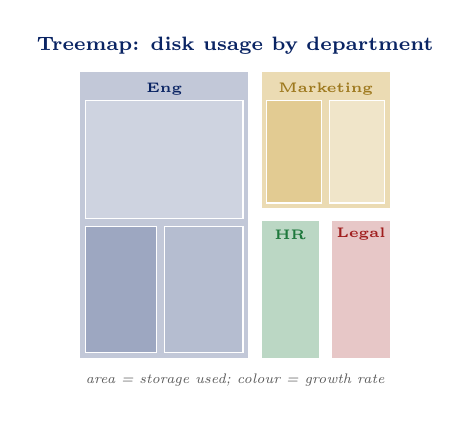
\begin{tikzpicture}
        % Treemap illustration (4 top-level groups)
        \node[font=\scriptsize\bfseries, text=PUNavy] at (2.0, 4.3)
              {Treemap: disk usage by department};

        % Group A — large
        \draw[fill=PUNavy!25, draw=white, line width=2pt]
              (0, 0.3) rectangle (2.2, 4.0);
        \node[font=\tiny\bfseries, text=PUNavy] at (1.1, 3.75) {Eng};
        \draw[fill=PUNavy!40, draw=white]
              (0.1, 0.4) rectangle (1.0, 2.0);
        \draw[fill=PUNavy!30, draw=white]
              (1.1, 0.4) rectangle (2.1, 2.0);
        \draw[fill=PUNavy!20, draw=white]
              (0.1, 2.1) rectangle (2.1, 3.6);

        % Group B — medium
        \draw[fill=PUGold!35, draw=white, line width=2pt]
              (2.3, 2.2) rectangle (4.0, 4.0);
        \node[font=\tiny\bfseries, text=PUGold!80!black] at (3.15, 3.75)
              {Marketing};
        \draw[fill=PUGold!50, draw=white]
              (2.4, 2.3) rectangle (3.1, 3.6);
        \draw[fill=PUGold!25, draw=white]
              (3.2, 2.3) rectangle (3.9, 3.6);

        % Group C — small
        \draw[fill=PUGreen!30, draw=white, line width=2pt]
              (2.3, 0.3) rectangle (3.1, 2.1);
        \node[font=\tiny\bfseries, text=PUGreen] at (2.7, 1.9) {HR};

        % Group D — small
        \draw[fill=PURed!25, draw=white, line width=2pt]
              (3.2, 0.3) rectangle (4.0, 2.1);
        \node[font=\tiny\bfseries, text=PURed] at (3.6, 1.9) {Legal};

        \node[font=\tiny\itshape, text=PUGray] at (2.0, 0.05)
              {area = storage used; colour = growth rate};
      \end{tikzpicture}
      \end{center}
      \vspace{4pt}
      \begin{alertblock}{Dynamic Queries}
        Shneiderman proposed \textbf{dynamic queries}: sliders and
        buttons that update the visualisation in $<$100~ms.
        This is the conceptual predecessor of Tableau's filter shelf
        and Grafana's variable dropdowns.
      \end{alertblock}
  \end{columns}
\end{frame}

%----------------------------------------------------------------
\begin{frame}{Impact Today — Tufte (1983) \& Shneiderman (1996)}
  \begin{columns}[T]
    \column{0.50\textwidth}
      \begin{block}{How These Works Shape Modern Tools}
        \renewcommand{\arraystretch}{1.2}
        \begin{tabular}{@{}p{2.5cm}p{4.2cm}@{}}
          \toprule
          \textbf{Concept} & \textbf{Modern instantiation} \\
          \midrule
          Data-ink ratio    & Tableau's ``Remove formatting''
                              one-click; Grafana's minimal theme \\
          Chartjunk removal & D3's default: no axes, no gridlines
                              (add only what you need) \\
          Small multiples   & Tableau's ``Pages'' shelf; Facet wrap
                              in ggplot2; \texttt{facet\_grid} in R \\
          Sparklines        & Grafana stat panel; Bloomberg terminal;
                              GitHub contribution heatmap \\
          Mantra            & Tableau's drill-down; Kibana's
                              overview → filter → inspect flow \\
          Treemap           & Tableau, Power BI, D3 \texttt{d3-hierarchy};
                              disk analysers \\
          Dynamic queries   & Tableau sliders; Grafana variables;
                              Observable's reactive cells \\
          \bottomrule
        \end{tabular}
      \end{block}

    \column{0.47\textwidth}
      \begin{exampleblock}{Stanford CS246 / CMU 15-721 Perspective}
        \begin{itemize}
          \item Stanford CS246 assigns Tufte as required reading
                for the \textbf{results communication} module —
                every data mining result is only as good as its
                visualisation
          \item CMU 15-721 uses Shneiderman's taxonomy to frame the
                \textbf{query interface design} for OLAP dashboards:
                a time-series drill-down is a 1-D $\to$ temporal
                transition in Shneiderman's taxonomy
          \item MIT 6.830 notes that Tufte's data-ink principle
                directly motivates \textbf{columnar storage}:
                retrieve only the columns (``data ink'') needed;
                ignore the rest (``chartjunk'')
        \end{itemize}
      \end{exampleblock}
      \vspace{4pt}
      \begin{alertblock}{CLO3 Connection}
        Every Grafana/D3/Tableau deliverable in CLO3 assessments
        is graded against Tufte's data-ink ratio and Shneiderman's
        mantra — explicitly.
      \end{alertblock}
  \end{columns}
\end{frame}

%================================================================
\section{Case Study — New York Times Graphics Desk (2010--2022)}
%================================================================

%----------------------------------------------------------------
\begin{frame}{The NYT Graphics Desk: Data Journalism at Scale}
  \begin{columns}[T]
    \column{0.52\textwidth}
      \begin{block}{Who They Are and What They Build}
        The New York Times Graphics Desk is a team of
        $\approx$50 journalists, designers, and engineers who
        produce \textbf{interactive data visualisations} for
        nytimes.com — reaching \textbf{6 million readers per day}.\\[5pt]
        Notable members:
        \begin{itemize}
          \item \textbf{Mike Bostock} (2010--2015):
                invented \textbf{D3.js} while at NYT;
                used it to build the 2012 election maps
          \item \textbf{Amanda Cox}: Upshot editor;
                ``You Draw It'' participatory journalism pieces
          \item \textbf{Hannah Beachler}, \textbf{Josh Katz}:
                COVID-19 tracker team (2020--2022)
        \end{itemize}
        Their stack: \textbf{D3.js} for custom interactive graphics,
        \textbf{R + ggplot2} for exploratory analysis,
        \textbf{Python + pandas} for data processing,
        \textbf{Mapbox} for geographic layers,
        \textbf{ai2html} (Adobe Illustrator $\to$ HTML) for static.
      \end{block}

    \column{0.45\textwidth}
      \begin{center}
      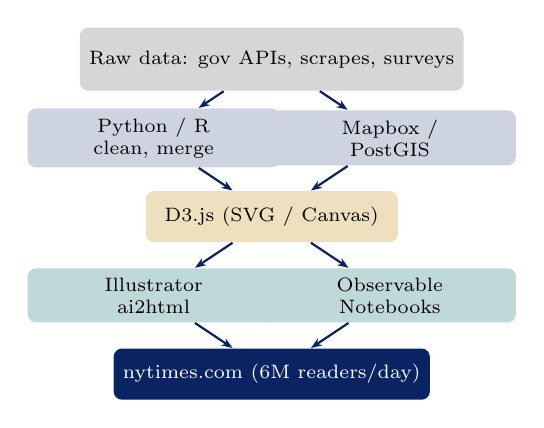
\begin{tikzpicture}[
          wb/.style={rectangle, rounded corners=3pt, minimum width=3.2cm,
                     minimum height=0.65cm, align=center, font=\scriptsize},
          arr/.style={-{Stealth[length=4pt]}, draw=PUNavy, thick}
        ]
        \node[wb, fill=PUGray!25, minimum width=4.0cm, minimum height=0.8cm]
              (raw) at (0, 4.4)
              {Raw data: gov APIs, scrapes, surveys};

        \node[wb, fill=PUNavy!20] (py)   at (-1.5, 3.4)
              {Python / R\\clean, merge};
        \node[wb, fill=PUNavy!20] (geo)  at (1.5,  3.4)
              {Mapbox /\\PostGIS};

        \node[wb, fill=PUGold!30] (d3)   at (0, 2.4)
              {D3.js (SVG / Canvas)};

        \node[wb, fill=PUTeal!25] (ai)   at (-1.5, 1.4)
              {Illustrator\\ai2html};
        \node[wb, fill=PUTeal!25] (obs)  at (1.5,  1.4)
              {Observable\\Notebooks};

        \node[wb, fill=PUNavy, text=white, minimum width=4.0cm]
              (pub) at (0, 0.4)
              {nytimes.com (6M readers/day)};

        \draw[arr] (raw) -- (py);
        \draw[arr] (raw) -- (geo);
        \draw[arr] (py)  -- (d3);
        \draw[arr] (geo) -- (d3);
        \draw[arr] (d3)  -- (ai);
        \draw[arr] (d3)  -- (obs);
        \draw[arr] (ai)  -- (pub);
        \draw[arr] (obs) -- (pub);
      \end{tikzpicture}
      \end{center}
  \end{columns}
\end{frame}

%----------------------------------------------------------------
\begin{frame}{Case: NYT COVID-19 Tracker (2020--2022)}
  \begin{columns}[T]
    \column{0.52\textwidth}
      \begin{block}{The Design Challenge}
        From March 2020 the NYT Graphics Desk built and maintained
        the most-read COVID-19 data tracker in the world:
        \begin{itemize}
          \item \textbf{Data sources}: Johns Hopkins CSSE, CDC,
                50 state health departments, county-level reporting
                — all with inconsistent schemas, missing values, and
                retroactive corrections
          \item \textbf{Daily pipeline}: Python scrapers
                $\to$ pandas cleaning $\to$ GitHub CSV repository
                $\to$ D3 charts auto-updated every hour
          \item \textbf{Charts produced}: 7-day rolling average line
                charts (Tufte small multiples for all 50 states),
                choropleth maps (county-level case rates),
                vaccination progress bar charts
          \item \textbf{Reach}: tracker page loaded
                \textbf{800 million times} in 2020;
                cited in CDC, WHO, and UK SAGE policy briefs
        \end{itemize}
      \end{block}

    \column{0.45\textwidth}
      \begin{block}{Tufte + Shneiderman Principles Applied}
        \begin{itemize}
          \item \textbf{Data-ink ratio}: no gridlines on case charts;
                only a light horizontal reference at the prior peak
          \item \textbf{Small multiples}: 50-state chart grid lets
                readers compare all states simultaneously without
                animation
          \item \textbf{Overview first}: national total at the top;
                state breakdown below; county detail on click
          \item \textbf{Zoom and filter}: state selector dropdown
                (Shneiderman dynamic query); date range slider
          \item \textbf{Details-on-demand}: hover tooltip shows
                exact date, count, and 7-day change
          \item \textbf{7-day rolling average}: reduces day-of-week
                reporting artefacts — a data quality decision
                encoded in the visual design
        \end{itemize}
      \end{block}
  \end{columns}
\end{frame}

%----------------------------------------------------------------
\begin{frame}{Lessons Learned \& Discussion Questions}
  \begin{columns}[T]
    \column{0.52\textwidth}
      \begin{block}{Key Lessons from the NYT Case}
        \begin{enumerate}
          \item \textbf{Data quality is a visualisation problem}:
                the NYT's biggest engineering effort was
                \emph{cleaning} data, not drawing charts;
                retroactive state corrections forced D3 charts to
                support negative bars (days where cases were revised down)
          \item \textbf{Accessibility is non-negotiable at 6M readers/day}:
                every chart had a data table alternative for
                screen readers; colour scales were tested for
                colour-blindness (deuteranopia, protanopia)
          \item \textbf{Small multiples beat animation}: the 50-state
                grid (Tufte small multiples) was more actionable than
                an animated map of spreading cases
          \item \textbf{Rolling averages are editorial decisions}:
                choosing 7-day vs.\ 14-day average changes
                \emph{what story the chart tells};
                these are journalistic choices with ethical weight
          \item \textbf{GitHub as data infrastructure}: publishing
                the raw CSV on GitHub enabled 1{,}000+ derivative
                dashboards worldwide within days
        \end{enumerate}
      \end{block}

    \column{0.45\textwidth}
      \begin{alertblock}{Discussion Questions \textmd{\tiny (CLO3)}}
        \begin{enumerate}
          \item A Grafana dashboard shows daily API error counts
                for a Big Data pipeline.
                Identify \textbf{three} Tufte violations in a
                dashboard that uses: a 3-D bar chart with a
                $y$-axis starting at 500, a heavy grid, and
                gradient fill colours.
                Redesign the chart applying data-ink principles.
                \textit{[CLO3 — Apply]}
          \item The NYT COVID tracker uses a \textbf{7-day rolling
                average} instead of raw daily counts.
                \textbf{(a)} What reporting artefact does this
                remove?
                \textbf{(b)} What real signal might a 7-day window
                mask that a 3-day window would reveal?
                Relate your answer to Shneiderman's ``zoom and filter.''
                \textit{[CLO3 — Analyse]}
          \item Design a \textbf{Shneiderman-compliant} interactive
                dashboard for a ride-sharing company's trip data
                (1M trips/day, 5 cities).
                Specify the overview view, the zoom/filter interactions,
                and the details-on-demand panel.
                Justify each design choice using the mantra.
                \textit{[CLO3 — Design]}
        \end{enumerate}
      \end{alertblock}
  \end{columns}
\end{frame}

%================================================================
\section{Live Exercise}
%================================================================

%----------------------------------------------------------------
\begin{frame}[fragile]{Live Exercise — D3.js Bar Chart with Tufte Styling}
  \begin{columns}[T]
    \column{0.50\textwidth}
      \begin{block}{Task (25 minutes, pairs)}
        Build a minimal D3.js bar chart that follows
        \textbf{Tufte's data-ink principles}:
        \begin{enumerate}\setlength\itemsep{1pt}
          \item No gridlines (or only a single light reference line)
          \item $y$-axis starts at 0
          \item No fill gradient — use a flat colour
          \item Tooltip on hover (Shneiderman: details-on-demand)
          \item Add a \textbf{sparkline} for each bar showing
                the 7-day trend
        \end{enumerate}
        \textbf{Dataset}: weekly Kafka message counts for
        5 topics (generate 7$\times$5 random values).\\[4pt]
        \textbf{Extension}: add a dropdown filter to select one
        topic and zoom into its 7-day line chart.
      \end{block}

    \column{0.47\textwidth}
      \begin{exampleblock}{HTML / D3 Skeleton}
        \scriptsize
        \begin{verbatim}
<!DOCTYPE html>
<meta charset="utf-8">
<style>
  .bar { fill: steelblue; }
  .bar:hover { fill: #b5651d; }
  .axis path, .axis line {
    stroke: #ccc; stroke-width: 0.5px; }
  .tooltip {
    position: absolute; background: #fff;
    border: 1px solid #ccc; padding: 6px;
    font-size: 11px; pointer-events: none; }
</style>
<body>
<script src=
  "https://d3js.org/d3.v7.min.js"></script>
<script>
const topics = ["orders","clicks",
                "errors","logins","search"];
const data = topics.map(t => ({
  topic: t,
  count: Math.floor(Math.random()*50000)
         + 10000
}));

const svg = d3.select("body").append("svg")
  .attr("width", 500).attr("height", 300);
const x = d3.scaleBand()
  .domain(data.map(d=>d.topic))
  .range([50,480]).padding(0.3);
const y = d3.scaleLinear()
  .domain([0, d3.max(data,d=>d.count)])
  .range([260, 20]);
svg.append("g").attr("transform","translate(0,260)")
  .call(d3.axisBottom(x));
svg.append("g").attr("transform","translate(50,0)")
  .call(d3.axisLeft(y).ticks(4));
svg.selectAll(".bar").data(data).join("rect")
  .attr("class","bar")
  .attr("x",d=>x(d.topic))
  .attr("y",d=>y(d.count))
  .attr("width",x.bandwidth())
  .attr("height",d=>260-y(d.count));
</script>
        \end{verbatim}
      \end{exampleblock}
  \end{columns}
\end{frame}

%================================================================
\section*{References}
%================================================================

%----------------------------------------------------------------
\begin{frame}{References}
  \begin{block}{Seminal Works}
    \begin{itemize}
      \item Tufte, E.~R. (1983; 2nd ed.\ 2001).
            \textit{The Visual Display of Quantitative Information.}
            Graphics Press.
      \item Shneiderman, B. (1996).
            The eyes have it: A task by data type taxonomy for
            information visualizations.
            \textit{Proc.\ IEEE Visual Languages}, 336--343.
    \end{itemize}
  \end{block}
  \vspace{4pt}
  \begin{block}{Textbooks \textmd{[SA], [TE], [LRU]}}
    \begin{itemize}
      \item \textbf{[SA]} Acharya, S., \& Chellappan, S. (2015).
            \textit{Big Data and Analytics}
            (Ch.~10 — Data Visualisation). Wiley.
      \item \textbf{[TE]} Erl, T., Khattak, W., \& Buhler, P. (2016).
            \textit{Big Data Fundamentals}
            (Ch.~11 — Visual Analytics). Prentice Hall.
      \item \textbf{[LRU]} Leskovec, J., Rajaraman, A., \&
            Ullman, J.~D. (2020).
            \textit{Mining of Massive Datasets}, 3rd ed.
            (Ch.~1 — Data and visualisation). Cambridge UP.
    \end{itemize}
  \end{block}
  \vspace{4pt}
  \begin{block}{Case Study Sources}
    \begin{itemize}
      \item Bostock, M., Ogievetsky, V., \& Heer, J. (2011).
            D$^3$: Data-driven documents.
            \textit{IEEE Trans.\ Visualization \& Computer Graphics,
            17}(12), 2301--2309.
      \item New York Times Graphics. (2020).
            \textit{Coronavirus in the U.S.: Latest Map and Case Count}.
            nytimes.com/interactive/2020/us/coronavirus-us-cases.html
    \end{itemize}
  \end{block}
\end{frame}

%----------------------------------------------------------------
\begin{frame}{Closing — Week 9, Part 2}
  \begin{columns}[T]
    \column{0.52\textwidth}
      \begin{block}{Key Takeaways}
        \begin{itemize}
          \item Tufte's \textbf{data-ink ratio} is a falsifiable metric:
                given two charts showing the same data, the one with
                the higher data-ink ratio communicates more efficiently.
                Apply it to every dashboard you build.
          \item Shneiderman's \textbf{mantra} (overview $\to$ zoom/filter
                $\to$ details) is a universal interaction design pattern
                — Tableau, Kibana, and D3 implement it differently
                but all adhere to it
          \item The NYT COVID tracker proved that \textbf{data quality
                is the invisible half of data visualisation}:
                the hardest engineering work was schema normalisation
                across 50 state health departments, not SVG rendering
          \item \textbf{D3.js} (created at NYT) is the direct
                application of Tufte's principle that the graphic
                designer must control every pixel of ink —
                D3 gives that control; Tableau and Grafana abstract it
        \end{itemize}
      \end{block}

    \column{0.45\textwidth}
      \begin{alertblock}{Quote of the Week}
        \begin{center}
        \large\itshape
        ``Above all else, show the data.''
        \end{center}
        \begin{flushright}
        \small --- Edward Tufte (1983)
        \end{flushright}
        \vspace{8pt}
        \begin{center}
        \large\itshape
        ``Overview first,\\
        zoom and filter,\\
        then details-on-demand.''
        \end{center}
        \begin{flushright}
        \small --- Ben Shneiderman (1996)
        \end{flushright}
      \end{alertblock}
      \vspace{4pt}
      \begin{exampleblock}{Part 1 Preview — Week 10}
        \textbf{Social Media, Time Series \& Health Data Analytics}\\[3pt]
        \begin{itemize}\setlength\itemsep{1pt}
          \item Twitter graph analytics
          \item Prophet time-series forecasting
          \item EHR pipelines \& FHIR integration
          \item CDC disease surveillance
        \end{itemize}
      \end{exampleblock}
  \end{columns}
\end{frame}

%=================================================================
\end{document}
%=================================================================
